\documentclass[11pt, a4paper]{article}
\usepackage[titlepage, fancysections, pagenumber]{polytechnique}
\usepackage[utf8]{inputenc}
\usepackage{multirow}
\usepackage{multicol}
\usepackage{array}
\usepackage{geometry}
\usepackage{indentfirst}
\usepackage{float}
\usepackage{listings}
\setlength{\parindent}{2em}
\usepackage{hyperref}
\usepackage{subfig}
\usepackage{emoji}
\setemojifont{Twemoji Mozilla}
\definecolor{Mycolor2}{rgb}{0.36, 0.54, 0.66}
\hypersetup{}


\lstset{frame=tb,
  language=python,
  aboveskip=3mm,
  belowskip=3mm,
  showstringspaces=false,
  columns=flexible,
  basicstyle={\small\ttfamily},
  numbers=none,
  numberstyle=\tiny\color{gray},
  keywordstyle=\color{blue},
  commentstyle=\color{dkgreen},
  breaklines=true,
  breakatwhitespace=true,
  tabsize=3
}

\usepackage[backend=biber]{biblatex}
\addbibresource{references.bib}

\title{Trending on tweet}
\subtitle{INF-583 Project}
\author{Kunhao \textsc{ZHENG}, Yujia \textsc{FU}}
\date{March 2021}

\begin{document}

\maketitle
\tableofcontents

\newpage
\section{Introduction}
Nowadays, social media has became an important way for people to get news. Compared to the mainstream media, it has larger coverage of events and shows the pressing issues discussed by citizens, can bring awareness and break the bubble. So the event detection in social media is meaningful. However, there is a lot of spam, publicity and false news. What's more, people use unstructured, short text and informal language. So the task of event detection is not easy.

In this project, we use PySpark(Apache Spark in Python) to perform trending detection and analyse on tweet. The data contains tweets in English and French in the first week of February 2020. There are 9 steps in total. Due to the limit of the computational capacity, we use one week of French tweets for the first 4 steps and one day of English tweets for the rest steps.

All related codes could be found on this github repository \href{https://github.com/DyeKuu/Trending-on-Twitter}{DyeKuu/Trending-on-Twitter}.


\section{Trending detection}
\subsection{Most frequent words}

\begin{lstlisting}[caption=Python Spark setup, label={spark setup}]
conf = SparkConf().setAppName("question1").setMaster("local[*]")
sc = SparkContext(conf=conf)
spark = SparkSession(sc)
lines = sc.textFile(','.join(FILES_PATH))
lines = lines.map(lambda line: json.loads(line))
\end{lstlisting}


In this part, we work on the French dataset. The code in Listing \ref{spark setup} shows how to set up Spark in Python, we load the data and convert them each to json format.

\begin{lstlisting}[caption=Filtering time range, label={filter time range}]
date_time_begin_str = 'Sat Feb 1 20:00:00 +0000 2020'
date_time_end_str = 'Sun Feb 2 20:00:00 +0000 2020'
date_time_pattern = '%a %b %d %H:%M:%S %z %Y'
def filter_time_range(s):
    curr_datetime = datetime.datetime.strptime(s['created_at'], date_time_pattern)
    return curr_datetime > date_time_begin_obj and curr_datetime < date_time_end_obj

words = lines.filter(filter_time_range).map(lambda d: d['text']).flatMap(lambda s: s.strip().split())
\end{lstlisting}

To find out the most frequent word in a certain time range, we define two variables to limit the time range, \texttt{date\_time\_begin\_str} and \texttt{date\_time\_end\_str} shown in Listing \ref{filter time range}. Then we define a function \texttt{filter\_time\_range} to filter all the tweets sent in the time range. Afterwards we do a flatmap to convert the texts into words.

\begin{lstlisting}[caption=Most frequent word, label={mfw}]
most_frequent_word = words.map(lambda x: (x, 1)).reduceByKey(lambda a, b: a + b).max(key=lambda x: x[1])
\end{lstlisting}

The code in Listing \ref{mfw} uses the map-reduce paradigm to count the occurrence of words. We first map each word to a tuple, which is itself along with unit count 1. Then we reduce all the tuple by key, which will take 2 objects with the same first element of tuple, and reduce them to 1 object using the rule define in \texttt{reduceByKey}. Finally, we extract the tuple with the biggest number of occurrence, thus the most frequent word. Note that before \texttt{max} the code realizes lazy-execution and will instantiate until the last step. We observe a quick execution during the intermediate steps.

The result is shown as follows.

\texttt{Most Frequent word from Sat Feb 1 20:00:00 +0000 2020 to Sun Feb 2 20:00:00 +0000 2020 is: RT with occurence 48409}


\subsection{Removing stopwords}
\label{mostFrequentWordsNoStop}
The result in the previous section is reasonable because when the tweet is in fact a retweet, it begins with the pattern ``RT @[username]:". So the word ``RT" will have a very high occurrence. We are going to remove the stop words then do again the word count.

We use the list of stop words in French provided on the Internet\footnote{https://countwordsfree.com/stopwords}. We found that the list is not complete in our specific case. So we extend the list by adding \texttt{['rt', ':', '?', ',', '.', '!','-', '\_', '/', '\guillemetleft', '\guillemetright', "c’est", "c'est", "j’ai", "j'ai"]}. Note that there are 2 encoding for the symbol single quote.

There are some fixed variables during the runtime, so it would be nice if we broadcast them. We broadcast notably 4 variables here: \texttt{date\_time\_begin\_obj, date\_time\_end\_obj, date\_time\_pattern, stop\_words}

Then we redo the same word count to the filtered words, with the result shown as follows.

\texttt{Most Frequent word from Sat Feb 1 20:00:00 +0000 2020 to Sun Feb 2 20:00:00 +0000 2020 is: faire with occurence 2678}

\subsection{Frequent seasonal words}
We consider that some of the tweets are written in the evening, where some words frequently appear but not in the daytime. To find out theses words, our approach is to split the tweets into 2 categories: night and day, according to its time. We use 2 constants to define the night time range. \texttt{NIGHT\_BEGIN = 18, NIGHT\_END = 6}. We also broadcast these 2 variables. The function in Listing \ref{isNight} shows how we retreive the night tweets.

\begin{minipage}{16cm}
\begin{lstlisting}[caption=Filter night tweets, label={isNight}]
def isNight(s):
    curr_hour = datetime.datetime.strptime(s['created_at'], date_time_pattern_broadcast.value).astimezone(local_timezone_broadcast.value).hour
    return curr_hour >= NIGHT_BEGIN_BROADCAST.value or curr_hour <= NIGHT_END_BROADCAST.value
\end{lstlisting}
\end{minipage}

We work all French tweets in this task. We separately count each word's occurrence in 2 categories, then we sort by the difference between the word count at night and that in day. Finally we take top 10 words who have the biggest difference. The code in Listing \ref{CWCD} shows all the logics discussed above. The \texttt{leftOuterJoin} will join 2 word count RDDs, and extending the second element of the tuples, for which the function \texttt{calDiffAndReverse} will calculate the difference. Note that the function also reverse the position to facilitate the \texttt{sortByKey}. 

\begin{lstlisting}[caption=Calculate word count difference, label={CWCD}]
def calDiffAndReverse(x):
    if x[1][1] is None:
        return (x[1][0], x[0])
    return (x[1][0] - x[1][1], x[0])
    
result = night_words_count.leftOuterJoin(day_words_count).map(
    calDiffAndReverse).sortByKey(False).take(10)
\end{lstlisting}

The result is shown as follows. We can observe that, the words with biggest difference word count between night and day are reasonable. Like ``vie", ``demain", ``soir", even ``\emoji{joy}". Maybe people need to relax during the night. 

\texttt{Top 10 most frequent words only in evening:
[(885, 'vie'), (808, 'demain'), (802, 'faire'), (741, 'oui'), (722, 'veux'), (681, '\emoji{joy}'), (599, 'soir'), (572, 'twitter'), (570, 't’es'), (562, 'meuf')]}



\subsection{Anomaly detection}
\label{anomalyDetection}

\subsubsection{Point by point Poisson Model}
\label{poissonModel}

To make anomaly detection in time serious, we use the Point-by-point Poisson Model introduced in the Technical report of tweet in 2015 \cite{trend2015}. We assume that the counts of tweets that contains a certain hashtag in a social data time series are Poisson-distributed around some average value, and then looking for unlikely counts according to the Poisson model shown below. 

\[P(c_i;v) = \frac{v^{c_i}\cdot e^{-v}}{c_i !}\] 

Where P is the probability of observing $c_i$ Tweets that contain a certain hashtag in the given time window, when the expected number of such Tweets is $v$. In our simple model, we use the count $c_{i-1}$ in the previous time window as the $v$. Then we check the unlikeliness of $c_i$ by looking at its distance with mean and the confidence interval of the count. We use a parameter $\eta$ to evaluate the unlikeliness.

\[c_i = \eta \cdot CI(\alpha, v) + v\]

Where $\alpha$ is the confidence level and CI() is the confidence interval. When $\eta$ exceeds a threshold $\eta_c$, we say that an anomaly is detected.

\subsubsection{Implementation on french tweet data set}
\label{implement}

Due to the limit of computational capacity, we use the smaller data set: tweets in French in the first week of February 2020. In order to get enough data, we want to choose a target hashtag with high total count. So first of all, using the code in Listing \ref{most frequent hashtags}, we count the number of the hashtags mentioned in the data set and list the 20 most frequent hashtags. The resulted hashtags are shown in Fig \ref{fig:topHashtag}.

\begin{lstlisting}[caption=Most Frequent hashtags, label={most frequent hashtags}]
def get_all_hashtags(s):
    hashtags = s['entities']['hashtags']
    res = []
    for hashtag in hashtags:
        res.append((hashtag['text'], 1))
    return res

frequent_hashtags = lines.flatMap(get_all_hashtags).reduceByKey(lambda a, b: a + b).sortBy(lambda x: x[1], ascending = False).take(20)
\end{lstlisting}


\begin{figure}[H]
    \centering
    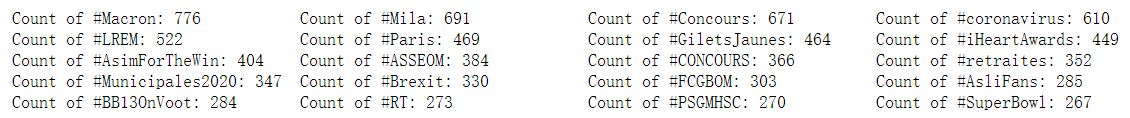
\includegraphics[width=1\textwidth]{images/top10_hashtags.png}
    \caption{Top 20 hashtags of tweets in French in the first week of February 2020}
    \label{fig:topHashtag}
\end{figure}

We choose '\#coronavirus' as our target hashtag. We set time window = 2h and the confidence level alpha = 0.99. With the code in Listing \ref{code:anomalyDetection}, we firstly filter the tweets which contain the hashtag '\#coronavirus'. Then we assign the time window to each tweet using the function 'get\_time\_period\_for\_row', note it as a property 'created\_at\_time\_period'. We count the number of '\#coronavirus' in each time interval, and calculate the $\eta$ with Poisson model introduced in \ref{poissonModel} using the function 'get\_eta'.

\begin{lstlisting}[caption=Anomaly detection of hashtag '\#coronavirus', label={code:anomalyDetection}]
tweet_with_hashtag = lines.filter(lambda s: filter_hashtag(s, target_hashtag)).map(lambda s: get_time_period_for_row(s, delta_time, date_time_begin_obj))
hashtag_trend = tweet_with_hashtag.map(lambda s: (s['created_at_time_period'], 1)).reduceByKey(lambda a, b: a + b)
hashtag_trend_df = spark.createDataFrame(hashtag_trend,schema=['t', 'hashtag_count']).toPandas()
hashtag_trend_df['eta1 (alpha = 0.99)'] = hashtag_trend_df.apply(lambda x: get_eta(x, alpha = 0.99), axis=1)
\end{lstlisting}

\begin{figure}[H]
    \centering
    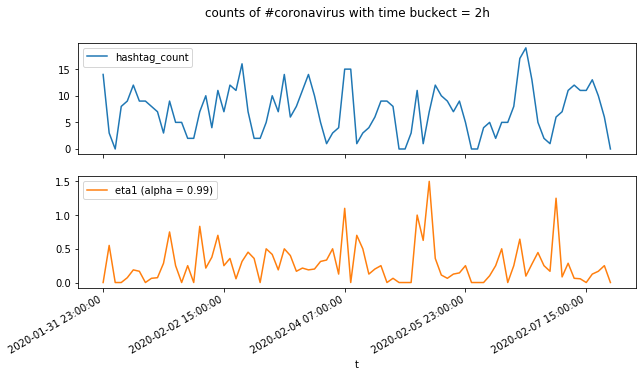
\includegraphics[width=0.8\textwidth]{images/countsAndEta_coronavirus_2h.png}
    \caption{Mentions of “\#coronavirus” per 2-hour intervals. For each point, $\eta$ is calculated based on the previous point, and plotted in yellow. In this case, $\alpha$ = 0.99.}
    \label{fig:countsAndEta_coronavirus_2h}
\end{figure}

With the threshold $\eta_c = 1$, we detect three time points with  anomaly: '2020-02-04 07:00:00', '2020-02-05 11:00:00', '2020-02-07 05:00:00'.

\subsubsection{Comparison of different parameters}

The anomaly detection depends on the choice of two parameters values: $\alpha$ and the time interval for a single data point. We choose different values of these parameters and analyse their influences.

\subsubsection*{Influence of $\alpha$}

In order to analyse the influence of $\alpha$, we use the same data set and parameters as in \ref{implement}, and change only the value of $\alpha$ into 0.6 and 0.3.

\begin{figure}[H]
    \centering
    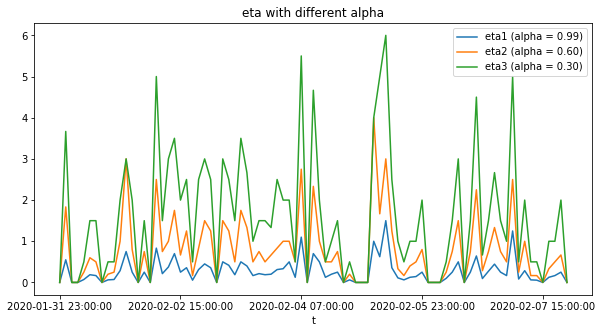
\includegraphics[width=0.6\textwidth]{images/eta_coronavirus_2h.png}
    \caption{$\eta$ of “\#coronavirus” per 2-hour intervals with different values of confidence level $\alpha$.}
    \label{fig:eta_coronavirus_2h}
\end{figure}

The $\eta$ of hashtag counts calculated with different $\alpha$ is shown in \ref{fig:eta_coronavirus_2h}. With a lower confidence level $\alpha$, the $\eta$ increases. That's because the confidence interval becomes smaller and the real count is more propabable to be far away from the confidence interval. So more trends are detected, but the noise also increases.

\subsubsection*{Influence of time interval}

In order to analyse the influence of time interval, we use the same data set and parameters as in \ref{implement}, and change only the value of time interval into 4h and 8h.

\begin{figure}[h]
    \centering
    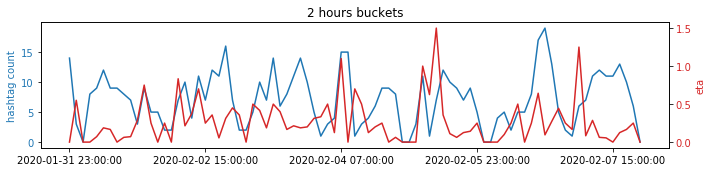
\includegraphics[width=0.7\textwidth]{images/coronavirus_2h.png}
    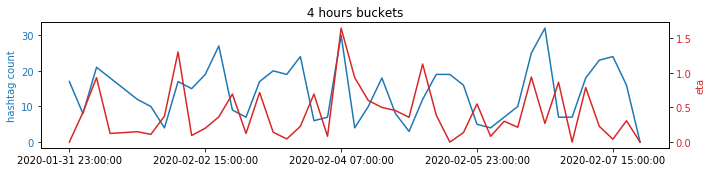
\includegraphics[width=0.7\textwidth]{images/coronavirus_4h.png}
    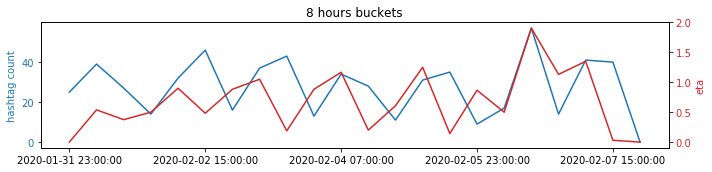
\includegraphics[width=0.7\textwidth]{images/coronavirus_8h.png}
    \caption{Mentions of “\#coronavirus” in different size of time interval. For each point, $\eta$ is calculated based on the previous point, and plotted in red. In this case, $\alpha$ = 0.99.}
    \label{fig:coronavirus_time_interval}
\end{figure}

The $\eta$ of hashtag counts calculated with different time intervals is shown in \ref{fig:coronavirus_time_interval}. With a smaller bin size, more trends are detected, but with a worse precision. Because when we use smaller time interval, we will catch more detailed trend of counts, some are noises. 

\subsection{Frequent words describing an event}

\label{frequentWordEvent}

In order to use some helpful English NLP libraries, we change into the English tweets data set in the following 4 steps. Since the data is large, we use the tweets in English on 02/01/2020. 

To extract the most frequent words describing an event, we detect event using the anomaly detection of one hashtag(as in \ref{anomalyDetection}), and then find out the most frequent words without stop words of the event related tweets in the event periods(as in \ref{mostFrequentWordsNoStop}).
\newpage

\begin{lstlisting}[caption=Frequent Words describing an event, label={code:requentWordsEvent}]
tweet_at_event = tweet_with_hashtag.filter(lambda s: s['created_at_time_period'] in event_intervals)
words_at_event = tweet_at_event.flatMap(lambda s: ps.stem(s['text']).strip().split())\
                .filter(lambda s: s not in stop_words)
most_frequent_words_at_event = words_at_event.map(lambda x: (x, 1))\
    .reduceByKey(lambda a, b: a + b)\
    .map(lambda s: (s[1], s[0]))\
    .sortByKey(False).take(20)

\end{lstlisting}

We choose the hashtag '\#BiggBoss13' to detect related events. We set the time interval = 1h, $\alpha = 0.99$, $\eta_c = 1.1$. After the anomaly detection, we detect three event periods. In the code at Listing \ref{code:requentWordsEvent}, 'tweet\_with\_hashtag' are  tweets with hashtag '\#BiggBoss13'. We filter them with the event periods to get tweets posted during the events, and we note them as 'tweet\_at\_event'. Then we extract the 20 most frequent words from 'tweet\_at\_event'. The resulted words that together describing the event '\#BiggBoss13' are shown in Fig \ref{fig:top20_words_bigboss}.

\begin{figure}[H]
    \centering
    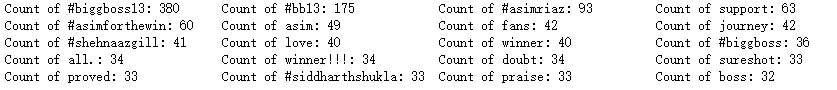
\includegraphics[width=1\textwidth]{images/top20_words_bigboss.png}
    \caption{Top 20 frequent words to describe the event '\#BiggBoss13'.}
    \label{fig:top20_words_bigboss}
\end{figure}


\subsection{Event time frame}

Now we want to get the time frame of the event detected in \ref{frequentWordEvent}. With the code in Listing \ref{code:timeFrame}, we firstly extract all the sentences for 'tweet\_at\_event' grouped by event period, and note them as 'sentences\_at\_event'. Then we make a summarize for sentences at each period with the function 'summarize'. In the summarize process, we clean the tweet text by the function 'filter\_tweet\_special\_text', which remove the words 'RT', the username indicator that starts with '\@' and the url start with 'http'. To do the summarize, we use the WordFrequency Algorithm: we count the word frequency in the text and calculate the score of each sentence by summing all its words' frequency, then take the two sentences with the highest scores to make a summarize. The summarize would be the introduction for one period in the event time frame. 

\begin{lstlisting}[caption=Time frame of an event, label={code:timeFrame}]
sentences_at_event = tweet_at_event.map(lambda s: (s['created_at_time_period'], s['text'])).reduceByKey(lambda a,b: a + '. ' + b)
sentences_at_event_list = sentences_at_event.collect()

summary_at_event = {}
for item in sentences_at_event_list:
    event_time = item[0]
    text = item[1]
    summary = summarize(text, n_top_sentence, tweet_stop_words = stop_words)
    summary_at_event[event_time] = summary
    print('At {}: \n {}'.format(event_time, summary))
    print()
    
def filter_tweet_special_text(word):
    if word == 'RT'or word.startswith('@') or word.startswith('http'):
        return False
    return True
\end{lstlisting}

The time frame for the '\#BiggBoss13' event is:

\begin{itemize}
    \item At 2020-02-01 07:00:00:  All praise  to the fans of Asim who have proved in his journey in \#BiggBoss13  that their love \& support has playe... Vikas Gupta entered \#BiggBoss13 in support of Sid  \& tried to play dirty game by dragging  innocent girl Sharuti T…... 
    \item At 2020-02-01 16:00:00:   \#BiggBoss13: Prior to \#SalmanKhan ’s \#WeekendKaVaar, \#AsimRiaz ’s fans show support \& trend \#AsimForTheWin’ -. Vikas Gupta entered \#BiggBoss13 in support of Sid  \& tried to play dirty game by dragging  innocent girl Sharuti T... 
    \item At 2020-02-01 17:00:00: \#BiggBoss13 \#BiggBoss \#Asim \#AsimRiaz \#Shukla \#SiddharthShukla \#ShehnazKaur…... Sana was a potential winner of \#BiggBoss13 but because of obsession with Siddhart Shukla she looks really bad, flipper \& no... 

\end{itemize}


\subsection{Location of event}

To get the location of event, we use the 'location' property of the tweet. With the code in Listing \ref{code:location}, we count the number of locations for all the 'tweet\_at\_event'. The most frequent locations of event '\#BiggBoss13' are shown in Fig \ref{fig:top20_locations_bigboss}. We can deduce that the event happened in India.

\begin{lstlisting}[caption=Location of an event, label={code:location}]
locations_at_event = tweet_at_event.filter(lambda s: 'user' in s and 'location' in s['user'])\
    .map(lambda s: (s['user']['location'], 1))\
    .reduceByKey(lambda a,b: a + b)\
    .sortBy(lambda x: x[1], ascending = False).take(20)
\end{lstlisting}

\begin{figure}[H]
    \centering
    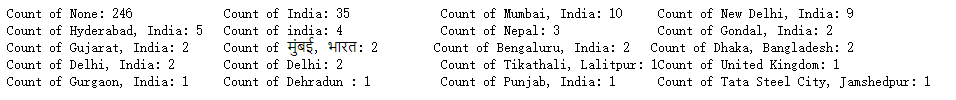
\includegraphics[width=1\textwidth]{images/top20_locations_bigboss.png}
    \caption{Top 20 frequent locations of the event '\#BiggBoss13'.}
    \label{fig:top20_locations_bigboss}
\end{figure}

\subsection{Sentiment around the event}


We use Vader(Valence Aware Dictionary for sEntiment Reasoning) \cite{gilbert2014vader} to analyse the sentiment of text. Vader is a library attuned to sentiments expressed in social media. It calculates a score between -1 to 1 for a sentence. A higher score means positive sentiment and a lower one means negative. 

With the function 'get\_sentiment\_scores' in Listing \ref{code:sentiment}, we do sentiment analysis for every sentence in the tweets of the event '\#BiggBoss13'. We firstly split the text into sentences, and then remove some special tweet characters with the function 'filter\_tweet\_special\_text'. Finally we do sentiment analyse with the Vader libarary. The histogram of sentiment scores for all the sentences are shown in Fig \ref{fig:sent1_bigboss}. Most of the tweets are neutral and there are more positive tweets than negative tweets.

\begin{lstlisting}[caption=Sentiment analysis of an event, label={code:sentiment}]
def get_sentiment_scores(text):
    sentiment_scores = []
    sentence_list = nltk.sent_tokenize(text)
    sentence_list = [newsent + '.' for sent in sentence_list for newsent in sent.split('\n') ] 
    sentence_list = [' '.join([word for word in sent.split(' ') if filter_tweet_special_text(word)]) for sent in sentence_list]
    analyzer = SentimentIntensityAnalyzer()
    for sentence in sentence_list:
        vs = analyzer.polarity_scores(sentence)
        sentiment_scores.append(vs['compound'])
    return sentiment_scores
\end{lstlisting}

\begin{figure}[H]
    \centering
    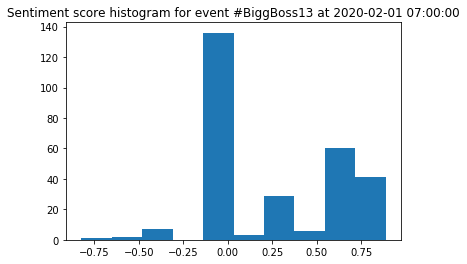
\includegraphics[width=0.7\textwidth]{images/sent1_bigboss.png}
    \caption{Histogram of sentiment scores of tweets in the event  '\#BiggBoss13'. The score is between -1 to 1. A higher score means positive sentiment and a lower one means negative.}
    \label{fig:sent1_bigboss}
\end{figure}


\subsection{Cluster tweets}
We work on a subset of the original English dataset. We take only the tweets in 2020-02-01. Then we first take a look at the top-20 hashtags. Then we extract the tweets only involving the top-5 hashtags, which correspond to top-5 events of that day. We will try to cluster these tweets.

To do tweets clustering, we must convert the tweets in text format to vectors. Due to the tweet's characteristics that it has a small length. Our first attempt is to use sentence embedding in FLAIR framework\cite{akbik2019flair} and plug it into the spark RDD map-reduce. However, we encountered mysterious error whether we broadcast the object for FLAIR framework or not. So we abandon this plan.

Our second attempt is to train a Word2Vec embedding from scratch based on our twitter dataset. This is more feasible because Spark has a bulit-in Word2Vec model framework.

\begin{lstlisting}[caption=data preprocessing, label={datapre}]
def clean_tweet(t: str):
    t = t.replace('\n','').strip()
    t = re.sub("(@[A-Za-z0-9]+)|([^0-9A-Za-z \t])|(\w+:\/\/\S+)"," ",t).split()
    if t[0] == 'RT':
        t = t[1:]
    return t
tweet_with_hashtag_cleaned = tweet_with_hashtag.map(lambda s: (clean_tweet(s[0]), s[1]))
\end{lstlisting}

The code in Listing \ref{datapre} shows how we do the data preprocesssing to feed in the Word2Vec model. Basically, we want to remove all the pattern like url, @[username], `RT' tag and hashtags. For example, if the tweet before is \texttt{'RT @Tha5SOSVote: 50 REPLIES = 50 VOTES \textbackslash n\textbackslash n\#iHeartAwards \#BestCoverSong \#DancingWithAStranger @5SOS https://t.co/C6LB3JhqmN'}, then we will expect it to become \texttt{['50', 'REPLIES', '50', 'VOTES', 'iHeartAwards', 'BestCoverSong', 'Dancing\\WithAStranger']} after the preprocessing. This is exactly done by the function \texttt{clean\_tweet}.

\begin{minipage}{16cm}
\begin{lstlisting}[caption=Training Word2Vec, label={w2v}]
from pyspark.ml.feature import Word2Vec
word2Vec = Word2Vec(vectorSize=2, minCount=0, inputCol="text", outputCol="result")
model = word2Vec.fit(tweet_with_hashtag_cleaned_df)
result = model.transform(tweet_with_hashtag_cleaned_df)
\end{lstlisting}
\end{minipage}

The code above trains a Word2Vec model with feature space dimension = 2. The reason is that we cannot afford a large computation cost and it is easier for visualization in dimesion = 2. To obtain the embedding of a sentence, the method \texttt{model.transform} automatically takes the average of word vector in a sentence and returns it as the embedding of the sentence. The model adds a column \texttt{result} to store the embedding in the original dataframe.

\begin{lstlisting}[caption=K-means Clustering, label={kmeans}]
from pyspark.ml.clustering import KMeans
kmeans = KMeans().setK(5).setSeed(1234).setFeaturesCol('result')
model = kmeans.fit(result.select('label', 'result'))
centers = model.clusterCenters()
transformed = model.transform(result.select('label', 'result'))
\end{lstlisting}

The code in Listing \ref{kmeans} shows that we use k-means to do clustering for the sentence vector. It will add a column \texttt{prediction} to store the predicted label.

\begin{figure}[ht]
    \centering
    \subfloat[\centering K-means clustering]{{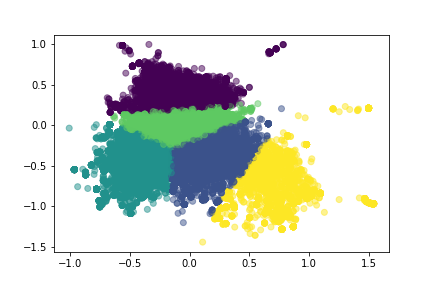
\includegraphics[width=0.45\textwidth]{images/kmeans-predict.png} }}
    \qquad
    \subfloat[\centering Ground Truth]{{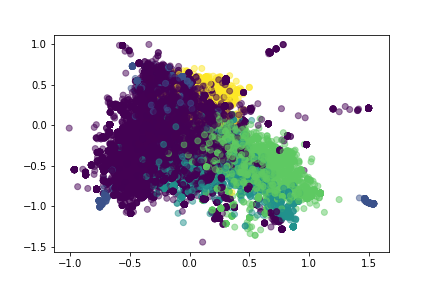
\includegraphics[width=0.45\textwidth]{images/kmeans-ground-truth.png} }}
    \caption{Comparison of clustering on top-5-event tweets}
    \label{k-means-top-5}
\end{figure}

Although k-means clustering can capture the cluster on the lower-right, it is not so satisfying. We think of several possible reasons:

\begin{itemize}
    \item The word vector space dimension is 2, thus too small. We cannot well separate sentences with different meaning.
    \item We observe that the tweet for the top event has roughly 10 times more than the second top event. Our dataset is not very balanced. Some hashtags are relavant.
    \item K-means is a linear model so it cannot deal with very well unlinear boundary.
\end{itemize}

To mitigate the limit of linear model, we tried Gaussian Mixture Model to do the clustering. The Figure \ref{GMM-top-5} shows that GMM is more suitable for clustering and it can capture both the boundary of the clusters on the upper-right and lower-right.

\begin{figure}[ht]
    \centering
    \subfloat[\centering GMM clustering]{{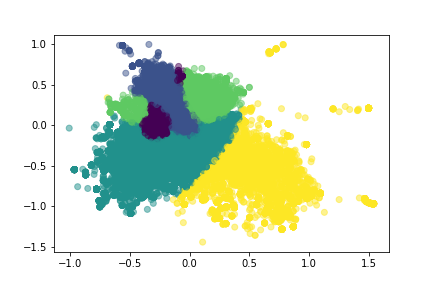
\includegraphics[width=0.40\textwidth]{images/GMM-predict.png} }}
    \qquad
    \subfloat[\centering Ground Truth]{{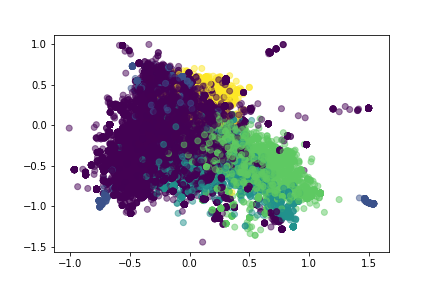
\includegraphics[width=0.40\textwidth]{images/kmeans-ground-truth.png} }}
    \caption{Comparison of clustering on top-5-event tweets}
    \label{GMM-top-5}
\end{figure}

We also observe that the hashtags that we have chosen may be highly relevant, like \#AsimForTheWin and \#AsimRiaz. We will choose another 5 topics semantically well separated and of the similar amount. We re-conduct all our experiments. It turns out that in dimension = 2, although both can capture some cluster structure, they are not very satisfying but still, GMM outperforms K-means.

\begin{figure}[H]
    \centering
    \subfloat[\centering Ground Truth]{{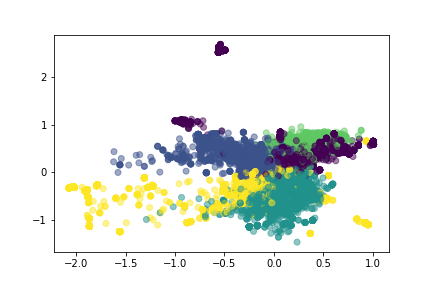
\includegraphics[width=0.4\textwidth]{images/new-ground-truth.png} }}
    \qquad
    \subfloat[\centering K-means clustering ]{{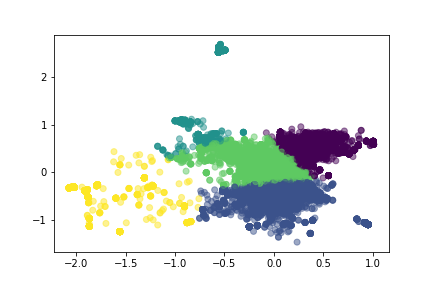
\includegraphics[width=0.4\textwidth]{images/kmeans-new-predict.png} }}
    \subfloat[\centering GMM clustering]{{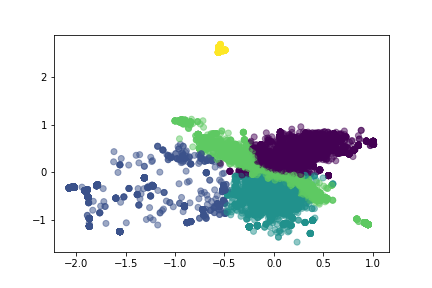
\includegraphics[width=0.4\textwidth]{images/GMM-new-predict.png} }}
    \caption{Comparison of clustering}
    \label{Final}
\end{figure}



\pagebreak

\printbibliography[
heading=bibintoc,
title={References}
]

\pagebreak

\end{document}
